\documentclass[preprint,12pt]{elsarticle}
% Draft 1 (2026-09-29). Target: Journal of Systems and Software (Elsevier); IST is the alternative.
% Compile: tectonic -X compile main.tex (or Overleaf). \todo{} marks what is still missing.
\usepackage{booktabs}
\usepackage{tabularx}
\usepackage{graphicx}
\usepackage{amsmath}
\usepackage{xcolor}
\usepackage[hidelinks]{hyperref}
\newcommand{\todo}[1]{\textcolor{red}{[TODO: #1]}}

\journal{Journal of Systems and Software}

\begin{document}
\begin{frontmatter}

\title{Revoked, But Not Gone: An Empirical Study of Access-Revocation Failures in Open-Source Web Software}

\author{Badeesorn Sittikong}
\address{King Mongkut's University of Technology Thonburi (KMUTT), Bangkok, Thailand}
% TODO: advisor / co-authors and affiliation

\begin{abstract}
Removing a user's access is supposed to take effect: a demoted administrator, a collaborator removed
from a project, or a deactivated account should lose what they could do before. We study how this goes
wrong in practice. From 35{,}979 reviewed advisories in the GitHub Advisory Database, we identify 229
access-revocation failures (187 in web applications) across 125 projects. Two independent coders labelled
each case with a codebook, a blind human re-code agrees with the adjudicated labels ($\kappa=0.96$), and a
stratified recall audit covers the whole database. We characterise
\emph{where} residual authority lives after revocation (its \emph{carrier}) and \emph{whether} a
test that starts from a clean state after the revocation could observe the failure. Most failures are
invisible to such tests: 77\% of web-application cases require state created \emph{before} the
revocation, such as a session, a token, an open connection, or an object the user created while authorised. Caches,
often named as the culprit, carry only 8 of 187 cases. Failures recur within projects, and their fixes
are repeatedly incomplete in a regular way: revocation is enforced per path, and fixes miss a revocation
trigger, a credential type, an entry path, or a response field. A source-only prototype that compares
cleanup across revocation paths of the same kind recovers one such incomplete fix in Gitea without
false alarms on that application. We release the dataset, codebook and scripts.
\end{abstract}

\begin{keyword}
access control \sep revocation \sep authorization \sep empirical study \sep security advisories \sep web applications
\end{keyword}
\end{frontmatter}

%======================================================================
\section{Introduction}
%======================================================================

Access control is usually tested as a snapshot: given a user and a policy, is this request allowed?
Revocation is different. It changes the policy while the system already holds state that was created
under the old policy, including sessions, issued tokens, open WebSocket connections, cached decisions,
scheduled jobs, and the ordinary data a user created while authorised (a watch on a repository, a
running stopwatch on an issue, a webhook). If any of that state keeps acting on the old authority, the
revocation is only partial.

Existing testing approaches mostly check authorisation from a clean state. ACtests~\cite{xiang2025actests}
tests configuration changes by comparing access decisions before and after a change in a fresh
environment, and notes that a cache service can be removed because it affects performance only.
REST fuzzers now carry access-policy oracles~\cite{sahin2026evomaster}, and model-based
approaches generate role-based access-control tests~\cite{xu2015rbac}. Work on AI agents studies revocation
for delegated and asynchronous work~\cite{zhu2026agentrevocation,shen2026agentmemory}. What is missing is
evidence about the failures themselves in ordinary web software. We lack answers to three questions: what carries residual
authority after a revocation, how much of it a clean-state test can see, and why fixes keep missing cases.

This paper answers these questions with a study of 229 revocation failures reported in the GitHub Advisory
Database~\cite{ghadvisorydb}. We ask:

\begin{description}
\item[RQ1] Where does residual authority live after a revocation?
\item[RQ2] How many failures can a test observe if it starts from a clean state after the revocation?
\item[RQ3] What is being revoked when these failures occur?
\item[RQ4] Why do fixes for revocation failures stay incomplete?
\end{description}

\paragraph{Contributions}
(1) A dataset of 229 access-revocation failures from 125 projects with a seven-way
carrier taxonomy, produced by two independent coders (relevance $\kappa=0.877$), validated by a blind human
re-code (relevance $\kappa=0.960$), and a recall audit covering the whole advisory database. (2) A clean-state-visibility measure: 77\% of web-application failures need
state created before the revocation, so testing from a clean state is structurally blind to them.
(3) Evidence that caches are a minority carrier (8 of 187), against a common intuition.
(4) A coverage account of incomplete fixes. Revocation is enforced per path, and recurring
failures are missing cells in a trigger$\times$carrier and entry-path$\times$check matrix. We support this
account with verbatim evidence from seven projects and with a source-only prototype that recovers one incomplete
fix. (5) A replication package.

%======================================================================
\section{Background and Related Work}
%======================================================================

\paragraph{Testing access control}
Model-based testing derives access-control tests from policy and behaviour models~\cite{xu2015rbac}.
ACtests~\cite{xiang2025actests} tests the impact of access-control configuration changes on deployed web
applications by forking a mini test environment. It reports 168 new vulnerabilities across 193 public
configurations. Sahin et al.\ add access-policy oracles to EvoMaster and generate executable
tests for REST APIs~\cite{sahin2026evomaster}. These approaches evaluate requests against the current
policy. Our RQ2 asks how much of the revocation problem remains outside that frame.

\paragraph{Sessions and logout}
Insufficient session expiration (CWE-613) and the failure to invalidate sessions or tokens at logout are
well known. OWASP ASVS contains requirements for them~\cite{owaspasvs}. Lamisa et al.\ audited the top one
million sites and found that 85\% of sites using JWTs fail to invalidate tokens upon logout and 51\% do not
terminate prior sessions after a password reset~\cite{loginplus}. We report this class for
completeness but do not claim it as new. Our contribution lies in the other revocation kinds and in the
carriers that are not sessions.

\paragraph{Revocation and consistency}
Global authorisation systems treat revocation as a consistency problem~\cite{pang2019zanzibar}. Recent work
studies revocation for long-running AI agents~\cite{zhu2026agentrevocation} and finds that agent-memory
systems do not enforce revocation labels~\cite{shen2026agentmemory}. We study the same phenomenon in
conventional web software, where derived state is spread across ordinary tables and code paths.

\paragraph{Authorisation bugs and incomplete fixes}
Kaur builds an empirical taxonomy of broken object-level authorisation from bug-bounty reports~\cite{kaur2026bola}.
Studies of incomplete security fixes examine multiple patches per CVE~\cite{zhang2026multipatch} and
incomplete fixes in the Linux kernel~\cite{liu2025kernelincomplete}. Our RQ4 gives a
revocation-specific account of why fixes remain incomplete.
\todo{Monitor for the ``incomplete-patch measurement study'' credited in GHSA-qf2f and cite it if published.}

%======================================================================
\section{Method}
%======================================================================

\subsection{Data source and candidate selection}
We cloned the \texttt{github-reviewed} tree of the GitHub Advisory Database on 29 September 2026
(35{,}979 advisories). A high-recall keyword filter over the summary and details fields selected
542 candidates. Its patterns cover revocation verbs, removal from teams, groups, projects and similar containers, deactivated or
deleted accounts, sessions that are not invalidated, stale permissions or tokens, and cached permission
decisions (\texttt{scripts/01\_filter.py}). We measured the filter's recall separately (Section~\ref{sec:recall}).
Table~\ref{tab:filter} lists the pattern families and how many candidates each matched. A candidate can
match several families.

\begin{table}[t]
\centering\small
\caption{Keyword-filter pattern families (matches overlap; 542 candidates in total).}
\label{tab:filter}
\begin{tabular}{lr}
\toprule
Pattern family (example) & Candidates \\
\midrule
Revocation verbs (\emph{revoke}, \emph{revocation}) & 303 \\
Cached permission or authorisation decision & 92 \\
Retained access (\emph{retain}, \emph{still have access}) & 50 \\
Session not invalidated or terminated & 44 \\
Token still valid after an event & 37 \\
Stale permission, session, token or role & 32 \\
Deactivated or deleted user still acting & 27 \\
\emph{Even after} removal, deletion, logout or change & 25 \\
Still able or allowed to & 20 \\
Removed from a container and still acting & 12 \\
No longer a member or authorised & 11 \\
Removed from team, group, project or organisation & 6 \\
Role or permission changed or lowered & 6 \\
After being removed, deleted or demoted & 1 \\
\bottomrule
\end{tabular}
\end{table}


\subsection{Codebook}
A case is \emph{relevant} if (i) a subject held some authority legitimately and that authority was
withdrawn, and (ii) the subject can still exercise part of it afterwards. Withdrawal includes
role or permission changes, removal from a group, account deactivation, credential or share-link
revocation, logout and password change. We exclude revocation checking in cryptographic
protocols and libraries (X.509 CRL/OCSP, SSH CA keys, PGP, verifiable credentials). We also exclude subjects who
never held the authority (for example ordinary IDOR), expiry by timeout, and single-use tokens that are not
consumed.

For relevant cases we code four fields. The \emph{carrier} records where residual authority lives:
\textsc{session}, \textsc{token}, \textsc{cache} (server-side), \textsc{connection} (a long-lived connection
opened before revocation), \textsc{data} (persistent residual grants or objects), \textsc{check} (the code
never checks the revoked state), or \textsc{async} (work queued before revocation). The \emph{clean-state
visibility} field records whether a test that starts after the revocation, with a new login and cold caches,
would observe the failure (yes, no, or cache-dependent). The remaining fields are the \emph{revocation kind} and
whether the software is a \emph{web application}. Two rules were added during adjudication (v1.1). R1: leaking data
the subject can no longer see counts as exercising withdrawn authority, even when only titles or
metadata leak. R2: a failure that needs an object the subject created before revocation is not clean-state
visible, even when the carrier is \textsc{data}.

Table~\ref{tab:carriers} gives each carrier with an example from the dataset.

\begin{table}[t]
\centering\small
\caption{Carriers of residual authority with one example each.}
\label{tab:carriers}
\footnotesize
\begin{tabularx}{\linewidth}{@{}l>{\raggedright\arraybackslash}p{3.4cm}>{\raggedright\arraybackslash}X@{}}
\toprule
Carrier & Residual authority lives in & Example (advisory) \\
\midrule
\textsc{token} & a credential issued before revocation & Vikunja link-share JWTs valid 72\,h after the share is deleted (GHSA-96q5-xm3p-7m84) \\
\textsc{session} & a login session established before revocation & pyLoad caches role and permission in the session at login (GHSA-66hx-chf7-3332) \\
\textsc{check} & a path that never consults the revoked state & Vikunja checks account status only at local login and token refresh (GHSA-94xm-jj8x-3cr4) \\
\textsc{data} & persistent grants or user-created objects & Gitea stopwatches started before revocation still expose issue titles (GHSA-j8xr-c56q-m8jj) \\
\textsc{cache} & a server-side cache of authorisation state & Budibase keeps revoked roles in a Redis user cache for up to 1\,h (GHSA-6vp2-6r7m-2jvx) \\
\textsc{connection} & a connection opened before revocation & Pterodactyl keeps SFTP connections after permissions are reduced (GHSA-8c39-xppg-479c) \\
\textsc{async} & work queued or configured before revocation & Open WebUI runs scheduled automations of a deactivated user (GHSA-mvx4-532p-xfm9) \\
\bottomrule
\end{tabularx}
\end{table}


\subsection{Coding procedure and agreement}
Two coders labelled all 542 candidates independently from the advisory text: Claude (Anthropic) and
Codex CLI (OpenAI, \texttt{gpt-5.6-sol}). Neither saw the other's labels. Agreement on relevance was
94.5\% ($\kappa=0.877$~\cite{cohen1960kappa}). On the 171 cases both coders marked relevant, $\kappa$ was
0.894 for carrier, 0.847 for clean-state visibility, 0.888 for kind, and 0.949 for the web-application flag. All 49
disagreements were adjudicated, each with a recorded reason (33 kept the first coder's label, 15 took the
second's, and 1 took neither). Most disagreements came from one ambiguity in the first codebook version, which rule R1 resolves.
To validate the labels, the first author re-coded a stratified blind sample of 100 candidates
(50 adjudicated relevant, drawn proportionally by carrier, and 50 not relevant) using the codebook alone, without access
to either coder's labels. Against the adjudicated labels \emph{as they stood before the re-code}, agreement on relevance
was 98\% ($\kappa=0.960$). On the 48 cases both marked relevant, $\kappa$ was 0.847 for carrier, 0.764 for
clean-state visibility, 0.947 for kind and 0.850 for the web-application flag. Of the 15 disagreements we then
revised 6 labels in the human coder's favour. In three of them the LLM coders had inferred a carrier that the
advisory text does not state, which violates the codebook's no-inference rule. These are now coded \emph{unclear}.
The other three changes were one relevance call, one visibility call and one kind call. We report agreement before these revisions, and
we added three clarifications to the codebook (v1.2).

\subsection{Recall audit}\label{sec:recall}
Because the keyword filter can miss cases, we audited the 35{,}437 non-candidate advisories by
stratified sampling in two rounds (Table~\ref{tab:recall}). Round~1 covered seven access-control CWEs. Round~2 covered the
rest, stratified by how many caught cases each CWE held. Codex coded the samples, and every ``relevant''
call was adjudicated (13 of 59 overturned, one of them a duplicate advisory). A blind check of 60 ``not relevant''
calls found no misses (95\% upper bound on the false-negative rate: 5\%). The audit recovered 46 missed cases.
The point estimate of the filter's recall is 0.73. The sampling lower bound is uninformative because
0 of 200 in the 27{,}013-advisory residual stratum cannot exclude much. That stratum holds only 6 of the 183 caught cases, however, so if the filter's recall there is similar to elsewhere, it hides one or two further cases.
All analyses below use the 229 cases (183 caught and 46 recovered).

\begin{table}[t]
\centering\small
\caption{Recall audit over non-candidate advisories. UB is a 95\% upper bound on missed cases (rule of three
when none were found).}
\label{tab:recall}
\resizebox{\linewidth}{!}{\begin{tabular}{lrrrrr}
\toprule
Stratum & Population & Sampled & Relevant & Est.\ missed & 95\% UB \\
\midrule
Seven CWEs, CWE-613 & 97 & 97 & 35 & 35 & 35 \\
Seven CWEs, other & 3,386 & 250 & 0 & 0 & 41 \\
CWE group A (287, 384, 281, ...) & 851 & 300 & 11 & 31 & 55 \\
CWE group B (200, 639, 522, ...) & 2,544 & 200 & 0 & 0 & 38 \\
No CWE & 1,546 & 150 & 0 & 0 & 31 \\
All other CWEs & 27,013 & 200 & 0 & 0 & 405 \\
\bottomrule
\end{tabular}
}
\end{table}

%======================================================================
\section{Results}
%======================================================================

\subsection{RQ1: Where does residual authority live?}
Figure~\ref{fig:carrier} and Table~\ref{tab:carrier} show the carriers for the 187 web-application cases.
Issued tokens (62) and sessions (55) dominate. They are followed by missing checks on some path (26), residual
data or objects (22), long-lived connections (9), caches (8) and queued work (2). In 3 cases the advisory says that
access persists without saying where, and we code the carrier as unclear. Caches are a minority carrier. Of the 8 cache
cases, 7 depend on whether the cache is per-session or shared.

\paragraph{Illustrative cases}
The carriers differ in \emph{how long} residual authority lasts and \emph{what} ends it. Token cases last
until expiry or indefinitely. Keycloak kept offline sessions valid after the \texttt{offline\_access} scope was
removed from a client, so refresh tokens continued to mint new access tokens (GHSA-895x-rfqp-jh5c).
Session cases last until logout or session expiry. Snipe-IT did not revoke active sessions when an account was
disabled (GHSA-636j-7x7r-gvw2). Connection cases last until the client reconnects. Argo CD's web terminal
kept accepting WebSocket messages after the user's \texttt{exec} permission was revoked (GHSA-v8wx-v5jq-qhhw),
and Open WebUI snapshotted the role into a Socket.IO session pool at connect time (GHSA-45m8-cpm2-3v65).
Cache cases last until the entry ages out: one hour in Budibase, up to three days for deleted API tokens in NocoDB
(GHSA-f76x-f9vj-92jv), and ``long after the configuration was changed'' in Jenkins' role-based strategy
plugin (GHSA-25g4-p347-x748). Data cases last indefinitely because nothing expires. Rancher left orphaned
role bindings after a project role was removed from a group (GHSA-28g7-896h-695v). Kimai let a user derive
new timesheets from historical entries in a project they no longer had access to (GHSA-c6w6-57jj-62vh).


\begin{figure}[t]
\centering
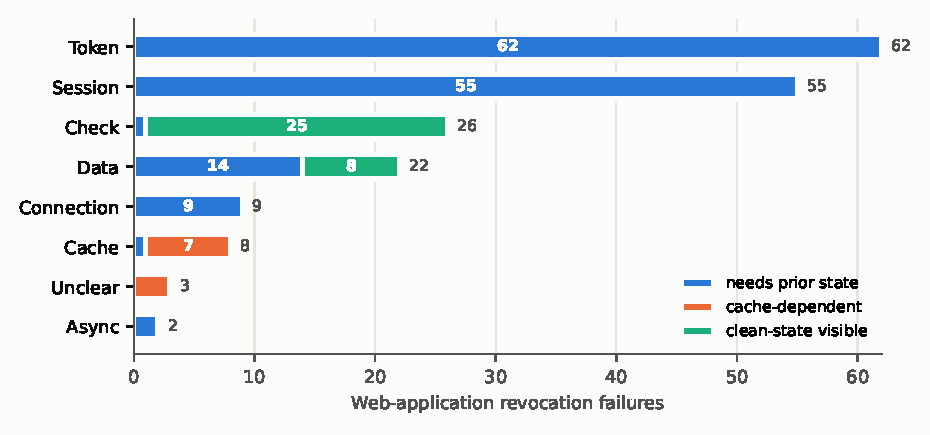
\includegraphics[width=\linewidth]{figs/carrier_visibility.pdf}
\caption{Carrier of residual authority and clean-state visibility for 187 web-application revocation failures.}
\label{fig:carrier}
\end{figure}

\begin{table}[t]
\centering\small
\caption{Carrier by clean-state visibility (web applications).}
\label{tab:carrier}
\begin{tabular}{lrrrr}
\toprule
Carrier & Needs prior state & Cache-dependent & Clean-state visible & Total \\
\midrule
Token & 62 & 0 & 0 & 62 \\
Session & 55 & 0 & 0 & 55 \\
Check & 1 & 0 & 25 & 26 \\
Data & 14 & 0 & 8 & 22 \\
Cache & 1 & 7 & 0 & 8 \\
Connection & 9 & 0 & 0 & 9 \\
Async & 2 & 0 & 0 & 2 \\
Unclear & 0 & 3 & 0 & 3 \\
\midrule
Total & 144 & 10 & 33 & 187 \\
\bottomrule
\end{tabular}

\end{table}

\subsection{RQ2: How much can a clean-state test see?}
Only 33 of 187 web-application failures (18\%) are visible to a test that starts after the revocation.
144 (77\%) strictly require state created before the revocation, and 10 more depend on cache design or are
unclear (154 in total, 82\%).
Every \textsc{token}, \textsc{session}, \textsc{connection} and \textsc{async} case needs prior state by
construction. The informative split is inside \textsc{data}: 8 cases are residual grants that a fresh
login still inherits, and 14 depend on an object the subject created while authorised. Examples are a running
stopwatch, an unread notification, a starred or watched repository, a webhook, a fork, or a historical
timesheet. A clean-state test starts without these objects and cannot see the leak.

\subsection{RQ3: What is being revoked?}
Table~\ref{tab:kind} crosses revocation kind with carrier. Logout and password change are the largest kind
(79 of 229) and live almost entirely in sessions and tokens, consistent with prior measurement~\cite{loginplus}.
Account deactivation or deletion (45) splits between tokens, sessions and missing checks. Permission changes (40)
and membership removal (13) are where residual data and objects concentrate.

\begin{table}[t]
\centering\small
\caption{Revocation kind by carrier (all 229 cases).}
\label{tab:kind}
\resizebox{\linewidth}{!}{\begin{tabular}{lrrrrrrrrr}
\toprule
Kind & Token & Session & Check & Data & Cache & Connection & Async & Unclear & Total \\
\midrule
Logout/Pwchange & 27 & 50 & 0 & 0 & 1 & 1 & 0 & 0 & 79 \\
Permission & 7 & 3 & 7 & 11 & 5 & 5 & 0 & 2 & 40 \\
Account & 15 & 10 & 17 & 1 & 0 & 1 & 1 & 0 & 45 \\
Credential & 19 & 2 & 2 & 0 & 8 & 4 & 0 & 0 & 35 \\
Membership & 0 & 1 & 1 & 8 & 0 & 1 & 1 & 1 & 13 \\
Other & 5 & 2 & 4 & 4 & 2 & 0 & 0 & 0 & 17 \\
\bottomrule
\end{tabular}
}
\end{table}

\paragraph{No weakness class captures revocation}
The 229 cases carry 44 distinct CWE identifiers. CWE-613 (Insufficient Session Expiration) is the most common,
yet it appears on only 107 cases (47\%). Eight CWEs are needed to cover 80\% of cases: CWE-613, 863, 287, 284, 384,
862, 285 and 269. A search for revocation failures by weakness class would therefore miss about half of them. This
is also why our candidate selection works on advisory text rather than CWE labels.


Figure~\ref{fig:year} shows advisories by publication year. The 2026 peak (98 cases through September)
coincides with growth in advisory volume and with batches from a few reporters. The 2022 peak partly reflects
the import of older CVEs: 32 of 229 advisories were published two or more years after their CVE year.
We therefore make no trend claim.

\begin{figure}[t]
\centering
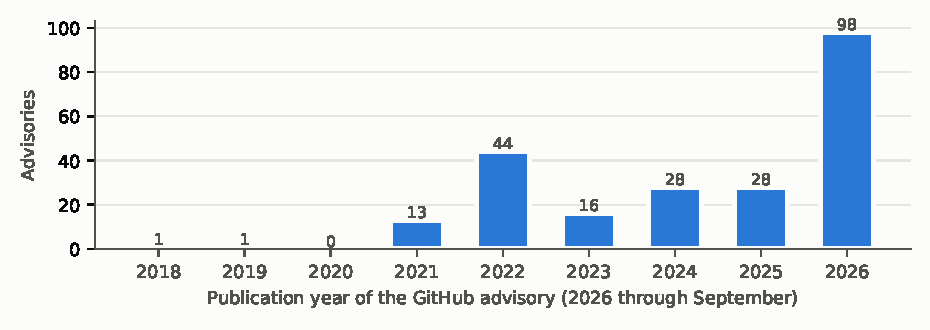
\includegraphics[width=\linewidth]{figs/by_year.pdf}
\caption{Relevant advisories by GitHub publication year (not vulnerability year).}
\label{fig:year}
\end{figure}

\subsection{RQ4: Why do fixes stay incomplete?}
Revocation failures recur within projects: 18 of 125 projects have three or more (Keycloak 12, Gitea 11,
OpenClaw 10, Open WebUI 9, Mattermost 8). Only 6 of 229 advisories state explicitly that an earlier fix was
incomplete. However, reading the patches of the 15 object-carried cases and the advisory text of the recurring
projects shows a regular structure.

A fix takes one of two strategies. \emph{Clean-up-on-revoke} deletes or disables derived state when
authority is withdrawn. \emph{Re-check-on-use} re-authorises the caller whenever derived state is read or
acted on. Each strategy carries a coverage obligation. Clean-up must be reached from every revocation trigger for
every carrier. Re-check must be applied on every entry or read path and to every field that renders protected
data. We observe four ways the obligation is missed:
\begin{enumerate}
\item \textbf{Revocation-path}: the cleanup is wired to one trigger only. In Gitea, the web path for making a repository
private clears watches but the REST path does not. In NocoDB, two of the three password flows delete refresh
tokens. In Open WebUI, only admin endpoints tear down sessions after a demotion, not the identity-provider sync
paths. In Airflow, the logout of two auth managers never reached token revocation.
\item \textbf{Carrier-type}: one trigger misses one kind of state. Gitea's API path clears stars but not watches,
and collaborator removal clears watches and assignments but not the collaborator's webhooks. NocoDB's OAuth-token
revocation was an empty stub. Mattermost's deactivation left personal access tokens valid.
\item \textbf{Entry/read-path}: a re-check is added to one endpoint only. Gitea's notification fix did not
cover the starred and tracked-time endpoints. Vikunja checked account status only at local login and token
refresh, not on API-token, CalDAV or OIDC authentication. Open WebUI enforced JWT revocation on HTTP but not on
its realtime surfaces.
\item \textbf{Field-level}: a re-check hides one field but not another. After Gitea's notification fix,
the repository field was nulled but the subject still exposed private titles and live activity.
\end{enumerate}
Table~\ref{tab:rq4} lists the evidence, quoted from advisory text or patch messages.

\begin{table}[t]
\centering\small
\caption{Evidence for the four incompleteness patterns (quotes from advisories and patches).}
\label{tab:rq4}
\footnotesize
\begin{tabularx}{\linewidth}{@{}l>{\raggedright\arraybackslash}p{3.3cm}>{\raggedright\arraybackslash}X@{}}
\toprule
Pattern & Project (advisory) & Evidence \\
\midrule
Revocation-path & Gitea (GHSA-q423-49rw-g9mh) & cleanup ``wired into \texttt{MakeRepoPrivate} only''; REST \texttt{updateRepository} not patched \\
Revocation-path & NocoDB (GHSA-r989-7g3j-wjhw) & \texttt{passwordChange}/\texttt{passwordReset} delete refresh tokens; \texttt{passwordForgot} does not \\
Revocation-path & Open WebUI (GHSA-wjwr-xfp9-r66p) & ``Only the admin user-management endpoints invalidated sessions'' \\
Revocation-path & Airflow (GHSA-vr7m-c6v4-8cx8) & auth-manager logout ``did not actually reach the underlying \texttt{revoke\_token()}'' \\
Revocation-path & OpenClaw (3 advisories) & device removal, token rotate, shared-token rotation each leave live WebSockets \\
Carrier-type & Gitea (GHSA-66m4-5jjr-2rg5) & collaborator removal clears watches and assignments, not webhooks \\
Carrier-type & NocoDB (GHSA-g72g-r7m4-9x4g) & \texttt{revokeAllOAuthTokensByUser} ``was an empty stub'' \\
Carrier-type & Mattermost (GHSA-mc2f-jgj6-6cp3) & deactivation ``fails to properly invalidate personal access tokens'' \\
Entry/read-path & Gitea (GHSA-qf2f-qh6p-7v89) & notification fix; ``two sibling endpoints \ldots still do not re-check'' \\
Entry/read-path & Vikunja (GHSA-94xm-jj8x-3cr4) & status ``checked in only two places''; API tokens, CalDAV, OIDC skip it \\
Entry/read-path & Open WebUI (GHSA-855v-hq7w-jmjw) & ``The realtime authentication surfaces do not perform this check'' \\
Field-level & Gitea (GHSA-44qc-pgvp-wx7v) & \texttt{repository} set to null, but \texttt{subject} still exposed \\
\bottomrule
\end{tabularx}
\end{table}

\subsection{A source-only coverage probe}
The first two patterns compare rows of a trigger$\times$carrier matrix, which suggests a static check. We
built a regex-level probe (\texttt{static/revcov.py}) for Gitea. It discovers ``artifact'' models (tables
that link a user to a repository or issue), computes which artifacts each revocation entry point cleans up,
and flags entry points of the same kind that clean up less than their siblings. We ran it on v1.26.2 and on v1.27.0 (after the fixes).
On v1.26.2 it raises exactly one cleanup flag, the known REST-path watch leak (GHSA-q423), and none on
v1.27.0. A second check for user-scoped read handlers that never use a permission result to filter
found the starred and subscriptions leak, which also disappears in v1.27.0. It is noisy on repository-scoped
routes. The probe misses the field-level leak, the webhook case (webhooks record no creator) and the fork case (a
repository-to-repository link). It is a feasibility result, not a tool evaluation.

%======================================================================
\section{Discussion}
%======================================================================

\paragraph{For testers and tool builders}
A clean-state oracle answers ``is this request allowed now?'', but revocation asks ``did everything created
before now stop acting on the old authority?''. Tests need to create state first (log in, issue tokens,
open sockets, create objects), revoke through every available trigger, and then probe every user-scoped read
path. The 229 cases can serve as a benchmark for such tools.

\paragraph{For developers}
Enumerate the carriers a revocation must reach and the triggers that can revoke, then check the matrix.
Prefer re-check-on-use at a single choke point, such as query-level conditions like an accessible-repository
filter, over per-endpoint checks. Where cleanup is necessary, route every trigger through one function.

\paragraph{A revocation coverage checklist}
The patterns in RQ4 suggest a simple review artefact. List the revocation \emph{triggers} as rows: role
change, group removal, account deactivation, deletion, credential revocation, logout, password change and
reset, visibility change, and identity-provider synchronisation. List the \emph{carriers} as columns: each
session store, each credential type, each long-lived connection, each cache, each scheduled or queued job, and
each table that links a user to a protected object. Every cell must be either handled at revocation time or
made harmless by a re-check at use. Of the 12 incompleteness cases in Table~\ref{tab:rq4}, 8 are an empty
cell in this matrix, and the other 4 are a read path or field without a re-check.

\paragraph{For state-preserving test generation}
A test generator that targets revocation has to invert the usual order. It creates authorised state
first (sessions, each credential type, sockets and user-created objects), revokes through each trigger, and then
exercises every user-scoped read path and connection. The oracle must know the application's intended
revocation latency. Several advisories describe bounded windows, such as Grafana's ``few seconds'' or cache TTLs, that
maintainers accepted or fixed case by case.

\paragraph{For advisory databases}
Revocation failures spread over 44 CWEs, and the most common one covers under half of them. A dedicated
weakness label or advisory tag for ``authority not withdrawn'' would make the class searchable.


%======================================================================
\section{Threats to Validity}
%======================================================================
\paragraph{Construct validity}
Our definition of revocation excludes expiry by timeout and cryptographic certificate revocation, and it includes
logout and password change. Other definitions would change the totals but not the carrier findings for
permission, membership and account revocation, which we report separately (Table~\ref{tab:kind}). Clean-state
visibility is judged from advisory text and is not observed by running tests.

\paragraph{Internal validity}
Both primary coders are LLMs, and one of them also performed adjudication. We mitigate this with an independent
second coder from a different vendor, recorded reasons for every adjudication, codebook rules made explicit,
and a blind human re-code of 100 cases (relevance $\kappa=0.960$). The re-code also showed that LLM
coders tend to infer mechanisms that the text does not state; we corrected the affected labels. The 46 recall-recovered cases carry a single coder's
carrier labels. Advisory text was truncated at 2{,}500 characters.

\paragraph{External validity}
We study reported failures in projects covered by the GitHub Advisory Database, which over-represents
ecosystems with package registries and projects that disclose actively. Reporting batches cluster: one Gitea
batch dominates the object-carried cases, and 2026 contributes 98 of 229 cases. We therefore make no claim about how prevalent
these failures are in deployed software, and no trend claim.

\paragraph{Reliability}
The recall point estimate is 0.73. The sampling lower bound is uninformative for the largest residual stratum.
The static probe was evaluated on one application with five known bugs and is not a tool evaluation.
The dataset, codebook, adjudication log and scripts are released so that others can re-derive every number.

%======================================================================
\section{Conclusion}
%======================================================================
Revocation fails where authority was copied before it was withdrawn. In 229 reported failures, most residual
authority lives in sessions, tokens, connections and user-created objects, which clean-state testing cannot see.
Caches matter far less than expected. Fixes stay incomplete because revocation is enforced per path. Making
that coverage explicit is a concrete target for both developers and tools.

\section*{Data availability}
\todo{Replication package: codebook, labels, adjudication log, recall samples, scripts, probe. Cite the
advisory snapshot date rather than redistributing the database.}

\section*{Declaration of generative AI use}
During this work the author used Claude (Anthropic) and Codex CLI (OpenAI) as two independent coders of
advisory text, as described in Section~3.3. Claude was also used to write analysis scripts, draft
parts of the manuscript and check references. All labels that enter the results were adjudicated with
recorded reasons, and a blind human re-code was performed. The author reviewed and edited all content and
takes full responsibility for the publication. \todo{Han to confirm wording against the current JSS policy.}

\bibliographystyle{elsarticle-num}
\bibliography{refs}
\end{document}
